% !TeX root = ../main-paper.tex
\section{OCR benchmark}
\label{sec:ocr-xp}

This section focuses on the evaluation of the performance of the three open-source OCR systems we selected, as described in \cref{sec:pipeline-summary}: Tesseract v4, Kraken and \peroocr.
The dataset used to perform this evaluation is composed of the $8,765$ entries (containing $424,764$ characters) from the dataset we previously introduced.
The single-column, cropped images of entries are used as input of each OCR system.
As the pages were previously deskewed, the text is mostly horizontal except for a few cases.
The expected output is the human transcription of these images provided in the dataset.
Before computing the Character Error Rate (CER) for each entry, each text prediction is normalised with the same basic rules as the ones used to post-process human transcription: dashes, quotes and character codes for glyphs like stars or hands are normalised.
% Regarding the charset of each OCR, Tesseract predicts characters covering a large portion of Latin script, \peroocr generates characters with a similar range, sometimes predicting some Cyrillic characters, and Kraken is constrained by its English model to predict only ASCII characters.


%\subsection{Results and discussion}

\begin{figure}

\subcaptionbox{}[.5\linewidth]{
\begin{tabular}{rlll}
\toprule
 & \peroocr  & Tesseract & Kraken \\    
\midrule
CER & 3.78\% & 6.56\% & 15.72\% \\  
\bottomrule
\end{tabular}
\bigskip

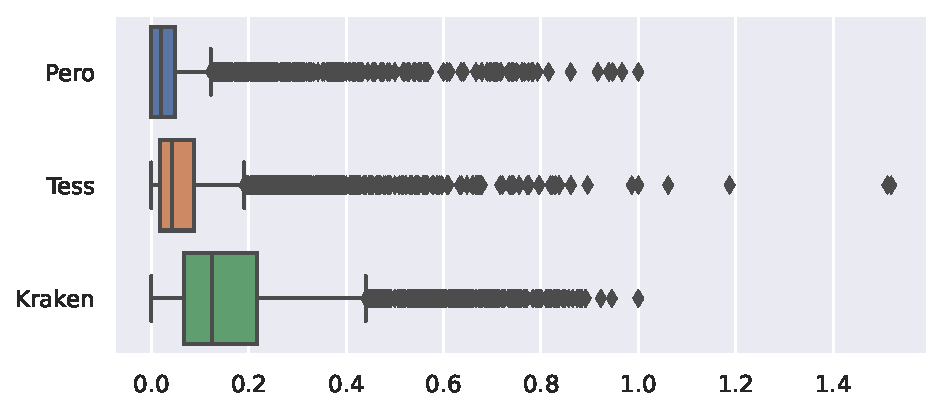
\includegraphics[width=\linewidth]{images/ocr-eval-2.pdf}
\medskip
}
\subcaptionbox{}[.5\linewidth]{
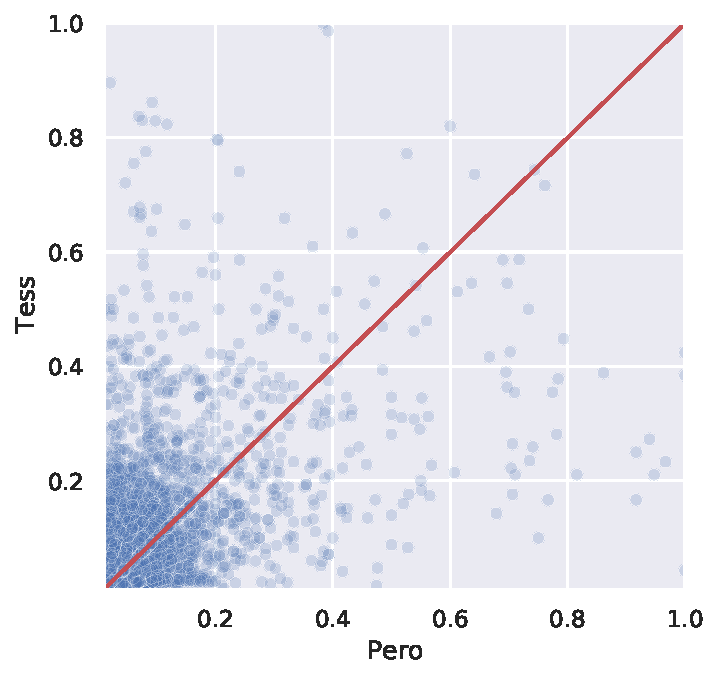
\includegraphics[width=\linewidth]{images/ocr-eval-1.pdf}
}
\caption{CER at entry-level for \peroocr, Kraken and Tesseract. (a) Global CER and distribution of the CER per entry. (b)
joint plot of the per-entry error rate showing that \peroocr and Tesseract do not fail on the same entries.}  
\label{fig.ocr-results}
\end{figure}
%
\Cref{fig.ocr-results} compares the performance of the OCR systems on our dataset. We can see Kraken's performance are
not as good as the two first OCR. This is partially due to the fact that the closest available model is for English text
and so it misses French specific symbols. On the other hand, even when using a French model trained on French 19th
documents, the performance does not increase (and relaxing the character matching rules does not help either). Tesseract and
\peroocr are performing better on this dataset ``out-of-the-box''. With no fine-tuning, \peroocr gets the best accuracy
with less than 4\% character errors. Many of them are even due to a bad line detection in case of multi-lines entries
and are not related to the OCR system itself. \Cref{fig.ocr-results} (b) shows that errors from the two best OCR are not
committed on the same entries (if so, all points would be on the diagonal line) and that combining the outputs of
\peroocr and Tesseract could improve the overall recognition quality. 
%In addition, we will not consider Kraken in the following NER experiments because its recognition rate is already too low.

